% Build twice here: pdflatex -interaction=nonstopmode -halt-on-error resume13An26w.tex
\documentclass[a4paper,10pt,pdflatex,ja=standard,jafont=ipaex-type1,
  magstyle=real,scale=1]{bxjsarticle}
\usepackage{lmodern}
\usepackage{amsmath,amssymb,mathtools}
\usepackage{geometry}
\geometry{reset,left=22mm,right=22mm,top=20mm,bottom=17mm,
  headheight=13pt,headsep=6mm,footskip=10mm}
\usepackage{xcolor}
\usepackage{enumitem}
\usepackage{array,booktabs,tabularx}
\usepackage{fancyhdr}
\usepackage{lastpage}
\usepackage{tikz}
\usetikzlibrary{arrows.meta,calc,decorations.pathreplacing}

\definecolor{ink}{HTML}{193A5C}
\definecolor{accent}{HTML}{237D82}
\definecolor{soft}{HTML}{EAF3F3}
\definecolor{muted}{HTML}{52616B}
\newcommand{\coursename}{解析学 II}
\newcommand{\handoutnumber}{13}
\pagestyle{fancy}
\fancyhf{}
\fancyhead[L]{\small\color{ink}\coursename{}・授業要約と演習}
\fancyhead[R]{\small\color{ink}第\handoutnumber 回}
\fancyfoot[C]{\small\color{ink}\thepage/\pageref{LastPage}}
\renewcommand{\headrulewidth}{0.3pt}
\setlength{\parindent}{0pt}
\setlength{\parskip}{2pt}
\setlength{\abovedisplayskip}{5pt}
\setlength{\belowdisplayskip}{5pt}
\setlength{\abovedisplayshortskip}{3pt}
\setlength{\belowdisplayshortskip}{4pt}
\setlist[itemize]{leftmargin=1.8em,itemsep=1pt,topsep=2pt,parsep=0pt}

\newcommand{\handouttitle}[1]{%
  \begin{center}
    {\Large\color{ink}#1}\par\vspace{3mm}
    {\color{accent}\rule{0.88\linewidth}{0.7pt}}
  \end{center}\vspace{-2mm}}
\newcommand{\handout}[2]{%
  \renewcommand{\handoutnumber}{#1}%
  \handouttitle{第#1回\quad #2}}
\newcommand{\topic}[1]{\par\vspace{5pt}%
  {\large\sffamily\mdseries\color{accent}#1}\par\vspace{2pt}}
\newcommand{\keybox}[1]{\par\vspace{3pt}\begingroup
  \setlength{\fboxsep}{4pt}%
  \colorbox{soft}{\parbox{\dimexpr\linewidth-2\fboxsep\relax}{\small #1}}%
  \endgroup\par\vspace{2pt}}
\newenvironment{problems}
  {\begin{enumerate}[leftmargin=2em,itemsep=3pt,topsep=3pt,parsep=0pt,
    font=\color{accent}]}
  {\end{enumerate}}


\newcommand{\examplelabel}[1]{{\sffamily\mdseries\color{ink}#1}}
\newcommand{\problemspace}{\par\vspace{5mm}}
\newcommand{\exercises}{%
  {\color{accent}\hrule height 0.7pt}\vspace{3pt}%
  \topic{演習問題（6題）}%
  {\small 領域と積分範囲を確認し、計算過程も書こう。図を描くと範囲を読み取りやすい。}\par}
\tikzset{
  handout diagram/.style={>={Stealth[length=3.2pt,width=3.2pt]},line join=round,
    every node/.style={font=\scriptsize,text=ink}},
  region/.style={fill=soft,draw=accent,semithick},
  slice/.style={accent,line width=1.8pt},
  guide/.style={muted,densely dashed,thin},
  axis/.style={->,ink,thin}}


% Review Q&A can also be used for actual student feedback when it is available.
\newcommand{\feedback}[2]{%
  \par\addvspace{8pt}\noindent\begin{minipage}{\linewidth}%
  {\color{ink}Q. #1}\par\vspace{2pt}%
  {\color{accent}A. }#2%
  \end{minipage}\par}

\begin{document}
\fontsize{10pt}{13.5pt}\selectfont
\setlength{\abovedisplayskip}{4pt}
\setlength{\belowdisplayskip}{4pt}
% Feedback section: add comments and responses here when available.
\fancyhead[L]{\small\color{ink}\coursename{}・フィードバック}
\handout{13}{前回のコメントへのフィードバック}
% \feedback{comment}{response}
\clearpage

% Previous small-test section: add the questions and solutions here.
\fancyhead[L]{\small\color{ink}\coursename{}・小テスト}
\fancyhead[R]{\small\color{ink}第12回}
\handouttitle{第12回\quad 小テスト}
% Questions and solutions are intentionally blank.
\clearpage

\fancyhead[L]{\small\color{ink}\coursename{}・授業要約と演習}
\fancyhead[R]{\small\color{ink}第\handoutnumber 回}
\handout{13}{面積分とグリーンの定理}\label{lesson-start}
\keybox{到達目標：スカラー場の面積分と流束を区別し、グリーンの定理で循環を面積分に直せる。
法線・境界の向き・場の定義域を、積分式と一緒に確認しよう。}

\topic{スカラー場の面積分とベクトル場の流束}
$D$ を有界な積分可能領域、$\phi,\vec F$ を $S$ 上連続とする。
正則な $C^1$ 級表示 $\vec r:D\to S$ は、内部で1対1とする。
$\vec N=\vec r_u\times\vec r_v$、$\vec n=\vec N/|\vec N|$ とおけば
$$
 \iint_S\phi\,dS=\iint_D\phi(\vec r(u,v))\,|\vec N|\,du\,dv,
$$
$$
 \iint_S\vec F\cdot\vec n\,dS
 =\iint_D\vec F(\vec r(u,v))\cdot\vec N\,du\,dv.
$$
スカラーの面積分は向きを変えても不変。流束は法線を反転すると符号が変わる。


\par\vspace{2pt}\noindent
\begin{minipage}[b]{0.48\linewidth}\centering
\begin{tikzpicture}[handout diagram,x=1cm,y=0.8cm]
\path[region] (0,0) -- (2.8,0.3) -- (3.4,1.7) -- (0.6,1.4) -- cycle;
 \fill[accent!22] (1.4,0.15) -- (2.8,0.3) -- (3.1,1) -- (1.7,0.85) -- cycle;
 \node at (1.4,0.65) {$\phi\,dS$};
 \node[above] at (2.2,1.8) {小さな面積に重みを掛ける};
 \draw[<->,ink] (0,-0.4) -- (2.8,-0.1) node[midway,below] {$dS$};
\end{tikzpicture}\par
{\small\color{muted}スカラー積分：向きを変えても同じ値}\par
\end{minipage}\hfill
\begin{minipage}[b]{0.48\linewidth}\centering
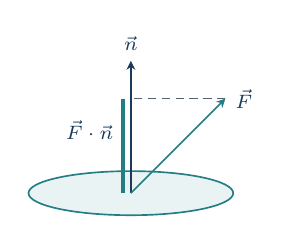
\begin{tikzpicture}[handout diagram,x=1cm,y=0.8cm]
\path[region] (0,0) ellipse (1.3 and 0.35);
 \draw[->,ink,semithick] (0,0) -- (0,2.1) node[above] {$\vec n$};
 \draw[->,accent,semithick] (0,0) -- (1.2,1.5) node[right] {$\vec F$};
 \draw[guide] (1.2,1.5) -- (0,1.5);
 \draw[slice] (-0.1,0) -- (-0.1,1.5);
 \node[left] at (-0.1,1) {$\vec F\cdot\vec n$};
\end{tikzpicture}\par
{\small\color{muted}流束：面を通り抜ける法線成分を足す}\par
\end{minipage}
\par\vspace{2pt}

\topic{グラフ上の計算}
$z=f(x,y)$ を上向きに取ると $\vec N=(-f_x,-f_y,1)$。
$\vec F=(P,Q,R)$ に対し、各成分を $z=f(x,y)$ で評価して
$$
 \iint_S\phi\,dS=\iint_D\phi(x,y,f)\sqrt{1+f_x^2+f_y^2}\,dx\,dy,
$$
$$
 \iint_S\vec F\cdot\vec n\,dS
 =\iint_D\bigl[-P(x,y,f)f_x-Q(x,y,f)f_y+R(x,y,f)\bigr]\,dx\,dy.
$$
後者では法線の大きさが面積要素と組み合わされており、平方根をもう一度掛けない。


\topic{グリーンの定理}
$D$ を区分的に滑らかな境界をもつ有界平面領域とし、
$P,Q$ は $\overline D$ を含む開集合で $C^1$ 級とする。
境界を領域が左に見える正の向きに取ると
$$
 \oint_{\partial D}(P\,dx+Q\,dy)
 =\iint_D(Q_x-P_y)\,dx\,dy.
$$
外側の境界は反時計回り、穴の境界は時計回りである。
場が領域内で特異点をもつときは、そのまま定理を適用できない。


\par\vspace{2pt}\noindent
\begin{minipage}[b]{0.98\linewidth}\centering
\begin{tikzpicture}[handout diagram,x=0.8cm,y=0.62cm]
\path[region,even odd rule] (0,0) circle (1.45) (0,0) circle (0.55);
 \draw[accent,->,semithick] (10:1.45) arc[start angle=10,end angle=160,radius=1.45];
 \draw[ink,->,semithick] (165:0.55) arc[start angle=165,end angle=15,radius=0.55];
 \node[right] at (2,0.8) {外側：反時計回り};
 \node[right] at (2,-0.25) {内側：時計回り};
 \node at (0,0) {穴};
\end{tikzpicture}\par
{\small\color{muted}どちらの境界でも、進むと領域が左に見える}\par
\end{minipage}
\par\vspace{2pt}

\newpage
% Keep the remaining summary in the upper half of page 2.
\noindent\begin{minipage}[b][\dimexpr0.5\textheight-\parskip\relax][t]{\linewidth}
\topic{長方形での証明の要点}
$D=[a,b]\times[c,d]$ の各辺を正の向きに積分する。
1変数の微分積分学の基本定理より
$$
 \begin{aligned}
 \oint_{\partial D}P\,dx
 &=\int_a^b(P(x,c)-P(x,d))\,dx=-\iint_DP_y\,dx\,dy,\\
 \oint_{\partial D}Q\,dy
 &=\int_c^d(Q(b,y)-Q(a,y))\,dy=\iint_DQ_x\,dx\,dy.
 \end{aligned}
$$
両式を足すと定理が得られる。領域を分けたとき、内部の共通辺の積分は逆向きとなって相殺する。


\par\vspace{2pt}\noindent
\begin{minipage}[b]{0.48\linewidth}\centering
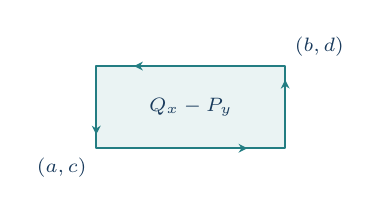
\begin{tikzpicture}[handout diagram,x=0.8cm,y=0.58cm]
\path[region] (0,0) rectangle (3,1.8);
 \draw[->,accent,semithick] (0.4,0) -- (2.4,0);
 \draw[->,accent,semithick] (3,0.3) -- (3,1.5);
 \draw[->,accent,semithick] (2.6,1.8) -- (0.6,1.8);
 \draw[->,accent,semithick] (0,1.5) -- (0,0.3);
 \node[below left] at (0,0) {$(a,c)$};
 \node[above right] at (3,1.8) {$(b,d)$};
 \node at (1.5,0.9) {$Q_x-P_y$};
\end{tikzpicture}\par
{\small\color{muted}長方形の4辺で基本定理を使う}\par
\end{minipage}\hfill
\begin{minipage}[b]{0.48\linewidth}\centering
\begin{tikzpicture}[handout diagram,x=0.8cm,y=0.58cm]
\path[region] (0,0) rectangle (1.5,1.8);
 \path[region] (1.5,0) rectangle (3,1.8);
 \draw[->,accent,semithick] (1.44,0.3) -- (1.44,1.5);
 \draw[->,ink,semithick] (1.56,1.5) -- (1.56,0.3);
 \node at (0.7,0.9) {$D_1$};
 \node at (2.3,0.9) {$D_2$};
 \node[above] at (1.5,2) {共通辺は逆向き};
\end{tikzpicture}\par
{\small\color{muted}隣り合う領域では、内部の辺が相殺する}\par
\end{minipage}
\par\vspace{2pt}

\topic{循環と面積への応用}
$\vec F=(-y,x)$ では $Q_x-P_y=2$。半径 $R$ の円周を反時計回りに回ると
$$
 \oint_{\partial D}(-y\,dx+x\,dy)=2\operatorname{Area}(D)=2\pi R^2.
$$
一般に、面積は境界上の積分でも表せる。
$$
 \operatorname{Area}(D)=\oint_{\partial D}x\,dy
 =-\oint_{\partial D}y\,dx
 =\frac12\oint_{\partial D}(x\,dy-y\,dx).
$$
\keybox{面積分では単位法線と面積要素を、グリーンの定理では境界の向きと場の定義域を確認する。}

\end{minipage}\par\nointerlineskip
% Keep the exercises and writing space in the lower half of page 2.
\noindent\begin{minipage}[b][0.5\textheight][t]{\linewidth}
\exercises
\begin{problems}
\item $S=\{(x,y,1):0\le x,y\le1\}$ を上向きに取る。$\iint_S(z+x)\,dS$ と、$\vec F=(x,y,z)$ の $S$ を通る流束を求めよ。
\problemspace

\item $\vec r(u,v)=(u\cos v,u\sin v,v)$（$0\le u\le1,\ 0\le v\le2\pi$）の外積を求めよ。$\iint_S1\,dS$ と $\vec F=(0,0,z)$ の流束を求めよ。向きは表示の外積による。
\problemspace

\item $D=[0,1]\times[0,2]$ の境界を正の向きに取る。$\oint_{\partial D}((x^2-y)\,dx+(x+y^2)\,dy)$ をグリーンの定理で求めよ。
\problemspace

\item 半径 $R>0$ の円周 $C$ を反時計回りに取る。$\oint_C(-y\,dx+x\,dy)$ を直接の媒介変数表示とグリーンの定理の両方で求めよ。
\problemspace

\item $a,b>0$、$x=a\cos t,\ y=b\sin t$（$0\le t\le2\pi$）で表される楕円の面積を、境界上の面積公式で求めよ。
\problemspace

\item 円環 $1\le x^2+y^2\le4$ 上の $\vec F=(-y/(x^2+y^2),x/(x^2+y^2))$ について、$Q_x-P_y$ と外側・内側の各循環を求めよ。境界全体でグリーンの定理を確かめ、原点を含む円板には直接適用できない理由を述べよ。
\problemspace
\end{problems}
\end{minipage}

\newpage
\handouttitle{第13回\quad 演習問題の解答}
{\small 設定した範囲と条件も確認しながら、計算を振り返ろう。}\par
\begin{problems}
\setlength{\itemsep}{7pt}
\item $z=1$ の平面では $dS=dx\,dy$、上向き法線は $(0,0,1)$。
$$
 \iint_S(z+x)\,dS=\int_0^1\int_0^1(1+x)\,dy\,dx=\frac32,\qquad
 \iint_S\vec F\cdot\vec n\,dS=\int_0^1\int_0^1 1\,dy\,dx=1.
$$

\item $\vec r_u=(\cos v,\sin v,0)$、$\vec r_v=(-u\sin v,u\cos v,1)$ より
$$
 \vec N=\vec r_u\times\vec r_v=(\sin v,-\cos v,u),\qquad |\vec N|=\sqrt{1+u^2}.
$$
したがって曲面積と流束はそれぞれ
$$
 \begin{aligned}
 \iint_S1\,dS
 &=2\pi\int_0^1\sqrt{1+u^2}\,du
 =\pi\bigl(\sqrt2+\log(1+\sqrt2)\bigr),\\
 \iint_S\vec F\cdot\vec n\,dS
 &=\int_0^{2\pi}\int_0^1 (0,0,v)\cdot\vec N\,du\,dv
 =\int_0^{2\pi}\frac v2\,dv=\pi^2.
 \end{aligned}
$$
面積では $|\vec N|$ を使い、流束では向きのある $\vec N$ をそのまま使う。

\item $P=x^2-y$、$Q=x+y^2$ より $Q_x-P_y=1-(-1)=2$。
グリーンの定理により、求める循環は $2\operatorname{Area}(D)=2\cdot2=4$。

\item $x=R\cos t$、$y=R\sin t$ とおくと
$$
 -y\,dx+x\,dy=R^2(\sin^2t+\cos^2t)\,dt=R^2\,dt.
$$
よって直接の積分は $\int_0^{2\pi}R^2\,dt=2\pi R^2$。
グリーンの定理でも $Q_x-P_y=2$ なので $2\pi R^2$ と一致する。

\item 表示は反時計回りなので、境界の面積公式を使える。
$$
 \operatorname{Area}(D)=\frac12\int_0^{2\pi}(x y'-y x')\,dt
 =\frac12\int_0^{2\pi}ab(\cos^2t+\sin^2t)\,dt=\pi ab.
$$

\item $r^2=x^2+y^2>0$ とおくと
$P_y=(y^2-x^2)/r^4=Q_x$、よって $Q_x-P_y=0$。
半径 $s$ の円を反時計回りに表示すると $-y\,dx/r^2+x\,dy/r^2=dt$ なので、
半径によらず循環は $2\pi$。円環の正の向きでは
$$
 \oint_{\text{外側}}\vec F\cdot d\vec r=2\pi,\qquad
 \oint_{\text{内側}}\vec F\cdot d\vec r=-2\pi.
$$
境界全体では和が0となり、$\iint_D0\,dA=0$ と一致する。
原点では場が定義されないため、原点を含む円板上では定理の $C^1$ 級の仮定を満たさない。
\end{problems}
\keybox{スカラー積分と流束では、外積の使い方が異なる。穴のある領域では、内側の境界も正しい向きで加えよう。}
\end{document}
